\chapter{Empirical Evaluation}\label{experiments}
In this chapter, we focus on the analysis of the different experiments that we have conducted
in order to assess and respond to our research questions that emerged from the motivation of this work. 

\section{Research Questions}
The fundamental part of this work focuses on incremental enumeration \acrshort{bt} in \acrshort{bg}. 
In spite of this, there are also other important areas for doing empirical analysis such as memory consumption, thread scheduling, and execution time.

Regarding that, we have asked ourselves the following research question that guides the empirical evaluation analysis, and we try to answer with the conducted experiments:
\begin{inparaenum}[\bf {\bf RQ}1\upshape)]
\label{res:bt:question}
    \item Does \acrshort{dpbt} generate incremental results regardless of the size of the graph?
    \item Does the type of query $Q$ impact on the execution of \acrshort{dpbt}?
    \item Does \acrshort{dpbt} follows a \emph{pay-as-you-go} model?
    \item Does \acrshort{dpbt} handle memory and threads efficiently?
\end{inparaenum}
  
\section{Experiments}
We have conducted different kinds of experiments to test our assumptions and verify the correctness of the implementation.
First, we have performed a \emph{Diefficiency Metric Analysis}~\cite{diefpaper} in order to assess the incremental capabilities of the implemented algorithm. 
Then we have performed a \emph{Benchmark Analysis} to identify how the algorithm varies depending on the type of query command selected for the user.
Finally, we have executed a \textit{Performance Analysis} in which we have to gather profiling data from \acrfull{ghc} for one of the graphs, 
to measure how the program performs regarding multithreading and memory allocation.

\subsection{Running Architecture}
All the experiments have been executed in the \emph{HPC Cluster at UPC}. The nodes architecture running in the cluster is $x86$ $64$ bits with a \textit{$24$-Core Intel(R) Xeon(R) CPU X5650} processor of $2.67$ GHz. 
Regarding memory, the allocated nodes have been requested from $40 GB$ up to $120 GB$ of RAM for the biggest \acrshort{dbpedia} graph. These machines also have $256\ KB$ of L2 cache memory, and $12\ MB$ of L3 cache.

\subsection{Haskell Setup}
Regarding specific libraries and compilations flags used on \acrshort{hs}, \acrshort{ghc} version $8.10.4$ has been used plus the following set of libraries: 
\begin{inparaenum}[]
      \item \mintinline{bash}{dyanmic-pipeline 0.3.2.0} \cite{dynamic-pipeline},
      \item \mintinline{bash}{bytestring 0.10.12.0} \cite{bytestring},
      \item \mintinline{bash}{containers 0.6.2.1} \cite{containers}, 
      \item \mintinline{bash}{relude 1.0.0.1} \cite{relude}
      \item and \mintinline{bash}{unagi-chan 0.4.1.3} \cite{unagi} 
  \end{inparaenum}. The use of \texttt{relude} library is because we disabled 
\mintinline{haskell}{Prelude} from the project with the language extension \mintinline{haskell}{NoImplicitPrelude} \cite{extensions}. 
We have compiled our program using \texttt{stack} version $2.5.1$ \cite{stack} with the following command and option flags\\ \mintinline{bash}{stack build --ghc-options "-threaded -O3 -rtsopts -with-rtsopts=-N"}.\footnote{For more information about package.yaml or cabal file please check https://github.com/jproyo/upc-miri-tfm/tree/main/bt-graph-dp}.

\subsection{DataSets}\label{data:set}

For all the experiments, the networks have been taken from Konect Networks~\cite{konect}. 
In this particular experiment setup, we have selected the following specific data sets that can be found here \cite{konect:2017:dbpedia-recordlabel,konect:2017:moreno_crime,konect:2017:opsahl-ucforum,konect:2017:wang-amazon}

\begin{table}[H]
  \centering
  \begin{tabular}{|p{0.25\linewidth}|c|c|c|c|c|}
    \hline
   \textbf{Network} & \textbf{$|U|$} & \textbf{$|L|$} & \textbf{$|E|$} & \textbf{Wedges} & \textbf{\#\acrshort{bt}} \\
   \hline
   Dbpedia & 18422 & 168338 & 233286 & $1.45 \times 10^8$ & $3.62 \times 10^8$\\
   \hline
   Moreno Crime & 829 & 551 & 1476 & 4816 & 211\\
   \hline
   Opsahl UC Forum  & 899 & 522 & 33720 & 174069 & $2.2 \times 10^7$ \\
   \hline
   Wang Amazon & 26112 & 799 & 29062 & $3.4 \times 10^6$ & 110269\\
   \hline
  \end{tabular}
 \caption{DataSet of selected \acrlong{bg}}
 \label{table:exp:data-set}
 \end{table}
 
The criteria for selecting those networks have followed the idea of conducting the analysis on one of the big networks~\cite{konect:2017:dbpedia-recordlabel} used on the \acrshort{bt} counting work~\cite{btcount}.
The rest of the networks, from the same data source~\cite{konect}, have been selected randomly but taking into consideration different sizes and topologies.

\subsection{Experiments Definition}\label{sub:exp:exp-def}
\paragraph{E1: Diefficiency Metric Analysis}\label{sub:sec:exp-1} In this experiment we asses the ability of \acrshort{dpbt} to generate results incrementally.
In order to do that, we use \acrfull{dm} Tool \emph{diefpy}~\cite{diefpy} which implements \emph{Diefficiency Metric}~\cite{diefpaper} measurement analysis.
Conducting this experiment, allows us to answer research questions [R1] and [R3] defined in \autoref{res:bt:question}. 

\paragraph{E2: Benchmark Analysis}\label{sub:sec:exp-2} In regards to benchmarking, we want to answer research question [R2] in order to know what is the impact of the type of command query $Q$ on enumerating \acrshort{bt}.
This also will indirectly answer [R3] because if a difference in the results based on the command is detected, we can deduce and answer [R3]. This was conducted using the same data sets and 
experiment setup as in \autoref{sub:sec:exp-1}, but removing \emph{\acrshort{dbpedia}} network and using \mintinline{shell}{criterion} \cite{criterion} benchmark tool.

\paragraph{E3: Performance Analysis}\label{sub:sec:exp-3} Finally we will take measurements on one network, to take measurements about the use of memory and threads on \acrshort{ghc}, using
\mintinline{shell}{ThreadScope} \cite{threadscope} and \mintinline{shell}{eventlog2html} \cite{eventlog2html} tools. 

\subsection{Experiments Data Setup}\label{sub:exp:exp-data-setup}
For the case of \nameref{sub:sec:exp-1} and \nameref{sub:sec:exp-2} we defined the following scenarios to conduct all the experiments regardless the network used.
We define \emph{low, high, and medium incidence level} as following:
\begin{inparaenum}
  \item[Low] A vertex or edge that is appearing in less than $5\%$ of the total number of edges
  \item[Medium] A vertex or edge that is appearing between $5\%-25\%$ of the total number of edges
  \item[Low] A vertex or edge that is appearing in more than $25\%$ of the total number of edges
\end{inparaenum}
The selection criteria are random in all cases, and for detecting the incidence level we have analyzed the data source and check how the vertex or edge is connected with the rest of the graph.

\begin{table}[H]
  \centering
  \begin{tabular}{|l|c|c|}
    \hline
   \textbf{Setup ID} & \textbf{Name} & \textbf{Search by}\\
   \hline
   E-H & Edge High & edge with high incidence \\
   \hline
   E-L & Edge Low & edge with low incidence \\
   \hline
   E-M & Edge Medium & edge with medium incidence \\
   \hline
   VL-H & $l \in L$ High & vertex in lower layer with high incidence \\
   \hline
   VL-L & $l \in L$ Low & vertex in lower layer with low incidence \\
   \hline
   VL-M & $l \in L$ Medium & vertex in lower layer with medium incidence \\
   \hline
   VU-H & $u \in U$ High & vertex in upper layer with high incidence \\
   \hline
   VU-L & $u \in U$ Low & vertex in upper layer with low incidence \\
   \hline
   VU-M & $u \in U$ Medium & vertex in upper layer with medium incidence \\
   \hline
  \end{tabular}
 \caption{Experiment Data Setup for experiments}
 \label{table:exp:data-setup}
 \end{table}

\section{\textbf{Observed Results Analysis}}\label{sec:discussion}
\subsection{Experiment: E1}\label{sub:sec:res:e1}
Regarding the results obtained by \acrshort{dm} tool, the data is presented in two different formats: the graphics that show 
how the different results are enumerated in each point of the time, and a radial graphic that shows the tension between aspects of the time measurement.
One important thing to point out about these graphs and data is that the time represents the number of nanoseconds elapsed to deliver that result from the moment the \acrshort{dpbt} finishes the execution of $\ac$ and it started executing $\ad$, so $\ad$ is able to start processing commands. 
Therefore time $0$ is equal to the start of $\ad$ execution.

\begin{figure}[!htb]
  \centering
  \begin{minipage}{0.5\textwidth}
   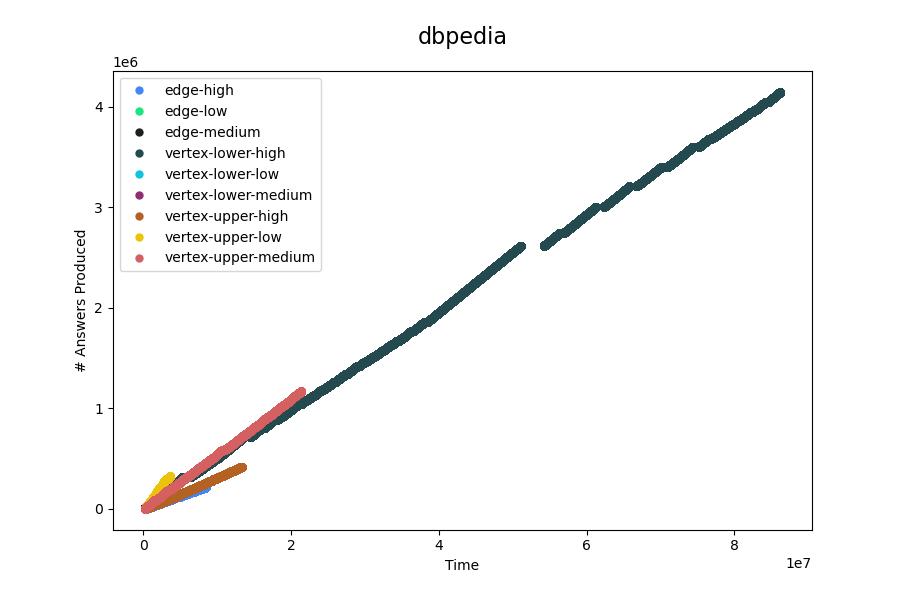
\includegraphics[width=1\linewidth, height=0.2\textheight]{experiments/diepfy/dbpedia.png}
    \caption{\acrshort{dm} Results: \acrshort{dbpedia}}
    \label{fig:dief:dbpedia}
  \end{minipage}%
  \begin{minipage}{0.5\textwidth}
   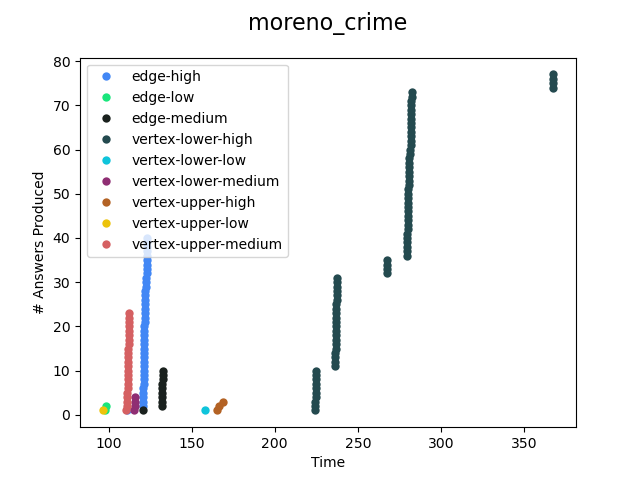
\includegraphics[width=1\linewidth, height=0.2\textheight]{experiments/diepfy/moreno_crime.png}
    \caption{\acrshort{dm} Results: Moreno Crime}
    \label{fig:dief:moreno}
  \end{minipage}
\end{figure}
%
\begin{figure}[!htb]
  \centering
  \begin{minipage}{0.5\textwidth}
   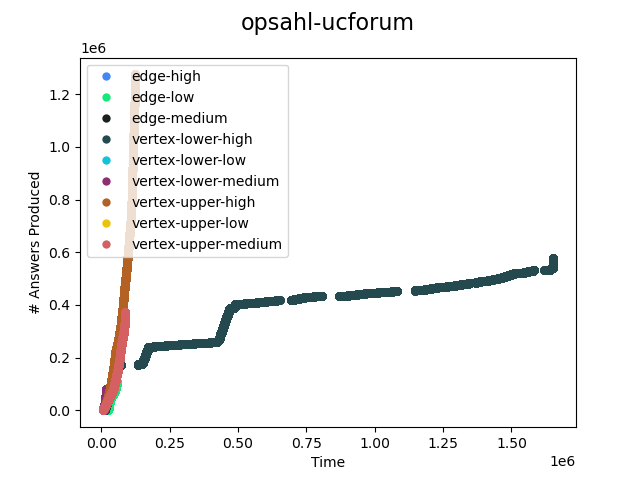
\includegraphics[width=1\linewidth, height=0.2\textheight]{experiments/diepfy/opsahl-ucforum.png}
    \caption{\acrshort{dm} Results: Opsahl UC Forum}
    \label{fig:dief:opsahl}
  \end{minipage}%
  \begin{minipage}{0.5\textwidth}
    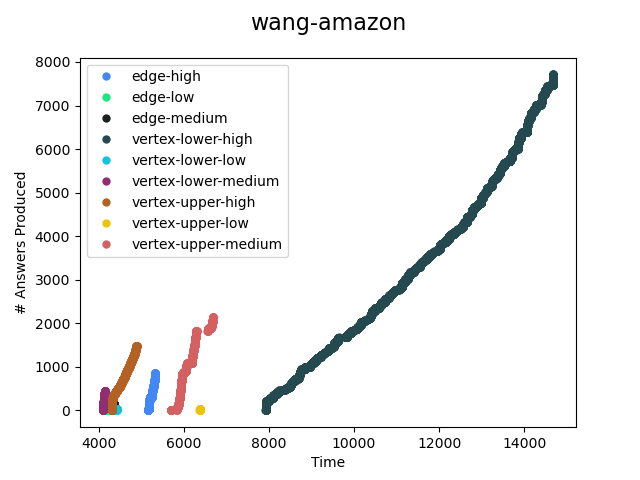
\includegraphics[width=1\linewidth, height=0.2\textheight]{experiments/diepfy/wang-amazon.png}
     \caption{\acrshort{dm} Results: Wang Amazon}
     \label{fig:dief:wang}
   \end{minipage}
 \end{figure}

As we can appreciate in the results above for all the data sets and for each of the experiments \acrshort{bt} are incrementally enumerated and deliver to the user. 
In all the cases above, we have seen how the experiment VL-H (see \autoref{table:exp:data-setup}) retrieves results incrementally better compare to the rest of the experiments. 
This is obvious since it is almost retrieving results at each moment of the execution and until the end. 
The behavior of this case can be explained because since we are aggregating bi-triangles based on some triple $(l_l,l_m,l_u)$ (see \dref{def:abt}) if the requested $l \in L$ matches with some of these triple elements, 
we need to enumerate all the $\ati$. Remember that VL-H stands for \emph{Vertex Lower with High Incidence}. Therefore there are many of them in the set $\ati$.

The only case that is not following this pattern is \autoref{fig:dief:opsahl}. That is explained because it is an outlier for this experiment.
Since the selection is random, we have detected that for this particular experiment, the selected vertex is not participating in many \acrshort{bt} as it should.
In fact, it can be seen that for VU-H, the selection was correct, but because of the speed of the retrieval, the incremental part cannot be appreciated properly\footnote{Check that the y-axis in the case of opsahl-ucforum and \acrshort{dbpedia} is $10^6$ scale as it is indicated on top of the graphic}. 

The case of Moreno Crime in \autoref{fig:dief:moreno} seems the least incremental of all the experiments. It could be explained by the fact of the topology of the graph, which is the smallest in all the graph metrics compared with the other three, both in terms of the number of \acrshort{bt} and the number of wedges.
Therefore it is extremely fast how the results are generated, and incremental results only can be appreciated in the vertices with high incidence.

\begin{figure}[!htb]
  \centering
  \begin{minipage}{0.5\textwidth}
   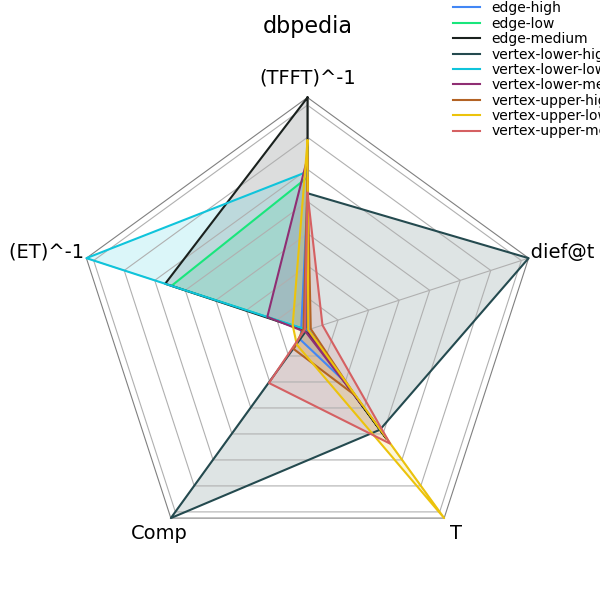
\includegraphics[width=1\linewidth, height=0.3\textheight]{experiments/diepfy/dbpedia_radial.png}
    \caption{\acrshort{dm} Results (Radial): \acrshort{dbpedia}}
    \label{fig:dief:dbpedia-radial}
  \end{minipage}%
  \begin{minipage}{0.5\textwidth}
   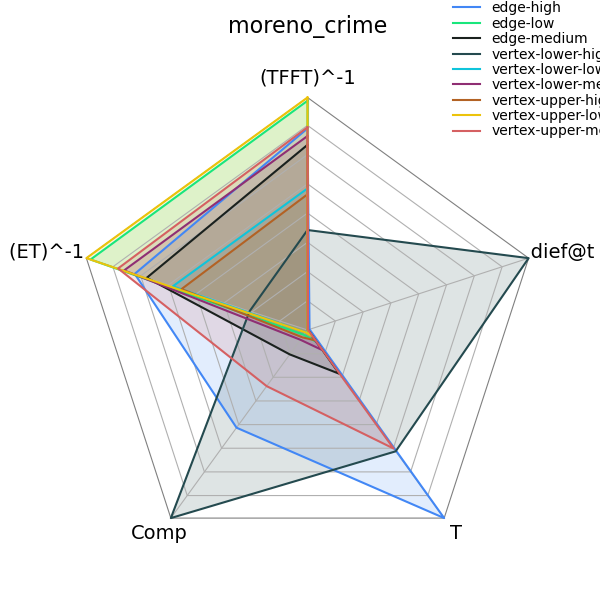
\includegraphics[width=1\linewidth, height=0.3\textheight]{experiments/diepfy/moreno_crime_radial.png}
    \caption{\acrshort{dm} Results (Radial): Moreno Crime}
    \label{fig:dief:moreno-radial}
  \end{minipage}
\end{figure}
%
\begin{figure}[!htb]
  \centering
  \begin{minipage}{0.5\textwidth}
   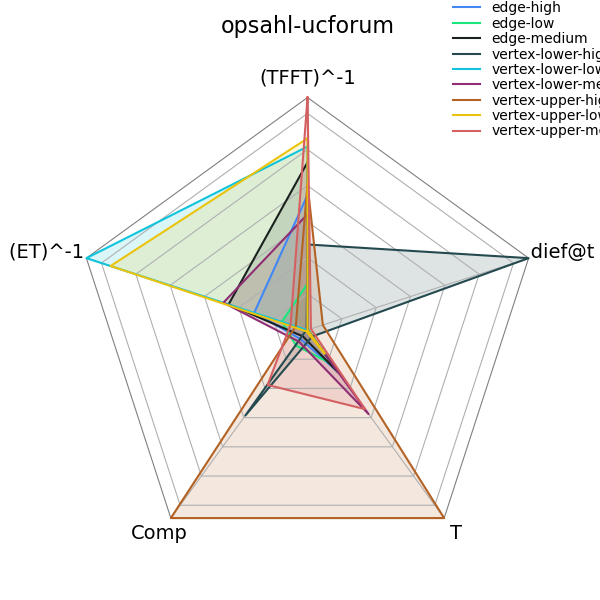
\includegraphics[width=1\linewidth, height=0.3\textheight]{experiments/diepfy/opsahl-ucforum_radial.png}
    \caption{\acrshort{dm} Results (Radial): Opsahl UC Forum}
    \label{fig:dief:opsahl-radial}
  \end{minipage}%
  \begin{minipage}{0.5\textwidth}
    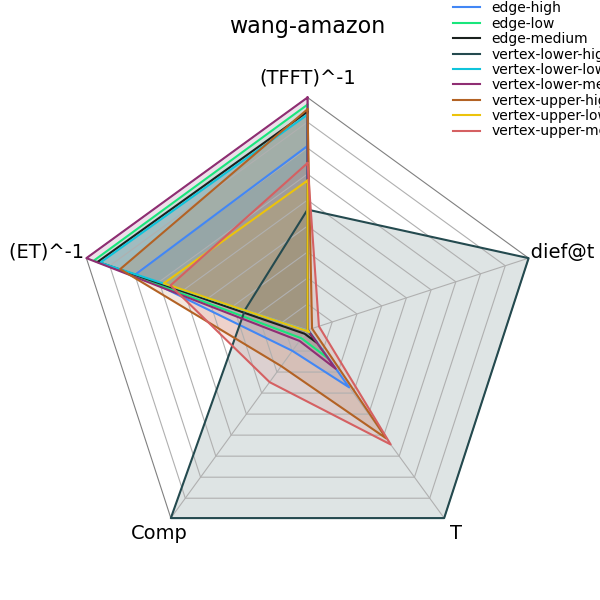
\includegraphics[width=1\linewidth, height=0.3\textheight]{experiments/diepfy/wang-amazon_radial.png}
     \caption{\acrshort{dm} Results (Radial): Wang Amazon}
     \label{fig:dief:wang-radial}
   \end{minipage}
 \end{figure}

These radial plots obtained from \acrshort{dm} shows the tension between \acrfull{dt} (higher better),
\acrfull{et}, \acrfull{tfft}, \acrfull{comp} and finally \acrfull{tt}. A perfect cover of each radial area with all the dimensions would
indicate a perfect solution with incremental delivery of results, completeness, throughput, etc. The important part to remark here that verifies
our deduction from the other graphics is that all the VL-H tension over \acrshort{dt} metrics are indicating that they are incremental on that part. 
The rest of the data setup experiments indicates that the level of throughput, completeness, and execution time is less than \acrfull{dt}, and the results can be delivered faster outlying incremental behavior. 
We know from the other graphics that is not true since there are more experiments setups that also deliver incremental results throughout time.

\paragraph{Conclusion E1} In conclusion, we are able to answer [R1] and asses that we have built an incremental algorithm for enumerating \acrlong{bt}. 
The same conclusion can be obtained regarding question [R3], verifying the \emph{pay-as-you-go} model because depending on the requirement of the user (command $Q$), the cost of obtaining results is faster or slower.

\subsection{Experiment: E2}\label{sub:sec:res:e2}
In the definition of \mintinline{shell}{criterion} tool \cite{criterion} it can be found that each benchmark is conducting running the same experiments many times (by default 100 each),
doing a statistical analysis on the execution time, eliminating outliers, and fitting a regression model that could explain that behavior. 
In this experiment, we have conducted the benchmark using all the networks and the same experiment setup presented in \autoref{data:set}. 
We have not considered for the benchmark analysis \acrshort{dbpedia} because of its size and the time taken to finish hundred of runs.

\begin{figure}[!htb]
  \begin{center}
     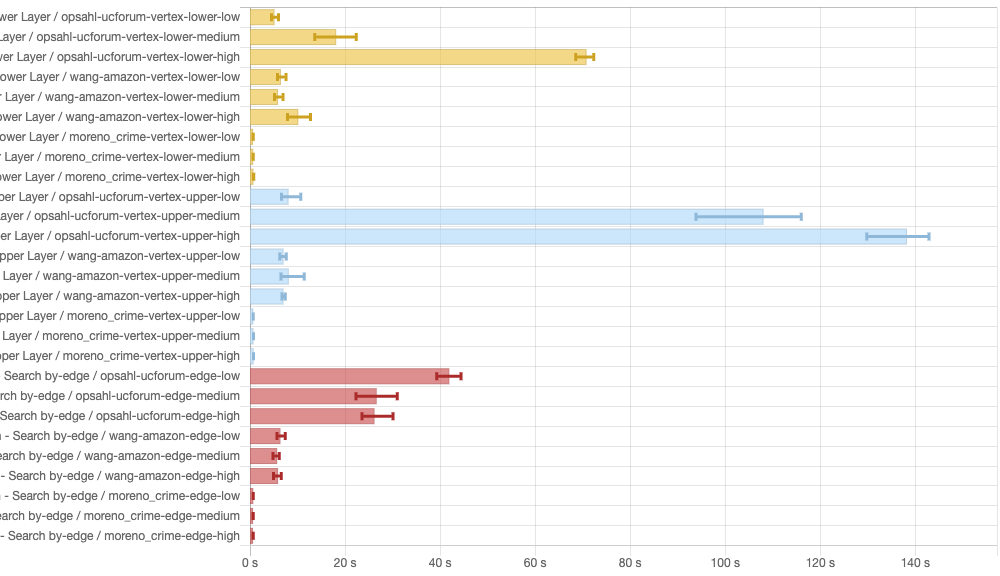
\includegraphics[width=1\textwidth] {experiments/bench_1}
       \end{center}
     \caption{Benchmark Results: Criterion Plot}
     \label{fig:exp:bench}
 \end{figure}

As it can be seen in \autoref{fig:exp:bench}, yellow bars are all the experiments related to Lower Layer vertices, blue bars are related to Upper Layer, and red bars are the experiments related to edges search. 
The longest bars are from network opsahl-ucforum, which we already know by \autoref{table:exp:data-set}, it is the biggest of three in terms of the number of \acrshort{bt} and wedges. So, it needs to enumerate more \acrshort{bt}. 
On the other hand, almost all the high incidence vertices and edges queries are taken longer as well. 
There is only one outlier which is E-H for opsahl-ucforum, which is explained by the random selection technique.

As we have explained, the tool fits a linear regression model with the observed empirical execution time.
We are not exposing the details of all these data for the regression model here, but the table can be found in \autoref{app:exp:bench}.
We can see from there, that there is only one case where the model could not fit the empirical data which is VU-L for opsahl-ucforum with an $R^2$ of $0.718$.
This could be explained by the execution time variance, with a lower bound of $600$ms, an average of	$2.43$s, and an upper bound of $3.18$s. 
This means that for some reason, this experiment was not stable or predictable from the execution time point of view.

Another benchmark that we have meassured, was the execution time of each experiment in order to compare them.

\begin{figure}[!htb]
  \begin{center}
     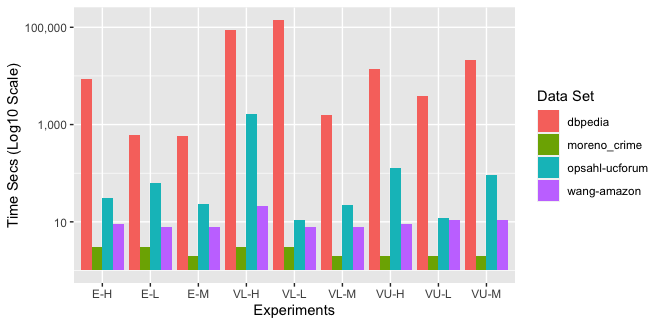
\includegraphics[width=1\textwidth] {experiments/execution_time_by_experiments}
       \end{center}
     \caption{Execution time results: Comparison between all setups}
     \label{fig:exp:bench:2}
 \end{figure}

Regarding \autoref{fig:exp:bench:2}, we have already seen in the other experiments that \acrshort{dbpedia} was the one which took more time in all experiments setups.
This is perfectly explained by the characteristics and topology of the graph. We can also see in this image that the experiments with higher incidence take more time to finalize the execution compared to the experiments with lower incidence. 

\paragraph{Conclusion E2} We can answer the question [R2] because it can clearly be seen in the benchmark analysis and in \autoref{fig:exp:bench:2} that as long as the user request for command queries $Q$ that have more incidence in the graph and participates in more \acrshort{bt},
the execution time increases. Therefore we are in a \emph{pay-as-you-go} model.

\subsection{Experiment: E3}\label{sub:sec:res:e3}
We can divide the analysis of this section into two: memory consumption and multithreading.

\paragraph{Multithreading} Regarding multithreading we have gather different moments of Moreno Crime network run.\footnote{We could not analyze bigger networks due to the huge amount of data gathered that make the program timeout running out of memory}.
As we can see in the overview execution in \autoref{fig:exp:perf:1} all the cores (8) are running MUT time in threads almost during the whole execution of the program.
\begin{wrapfigure}{r}{0.5\textwidth}
  \begin{center}
     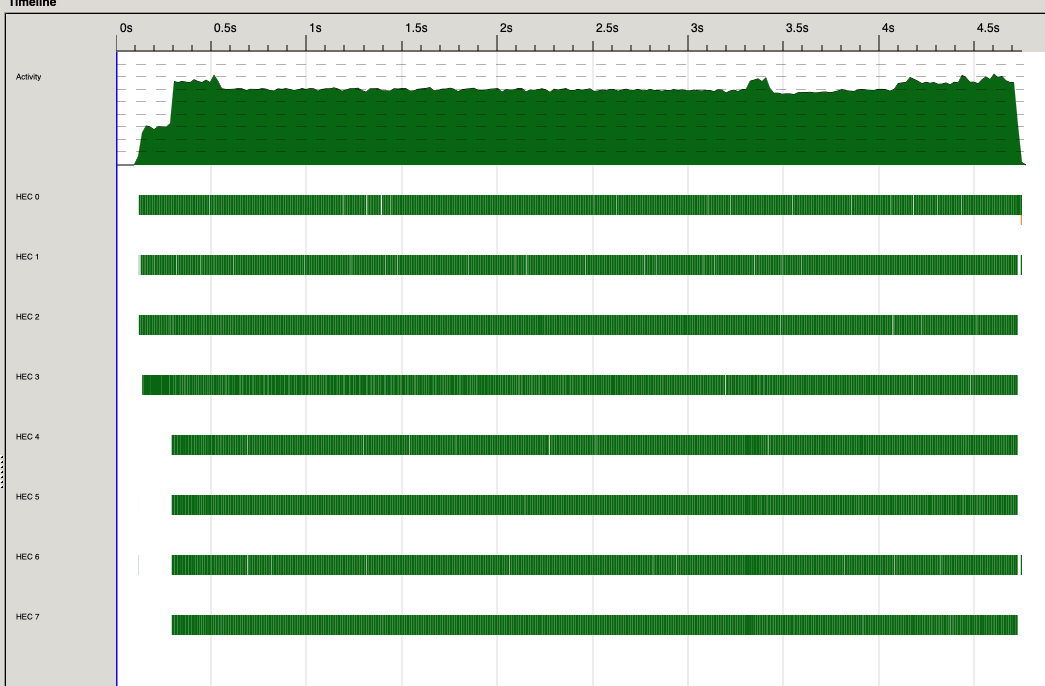
\includegraphics[width=0.48\textwidth] {experiments/thread/general_overview}
       \end{center}
     \caption{Thread Metrics: General overview}
     \label{fig:exp:perf:1}
 \end{wrapfigure}
This indicates that there are few GC pauses, and running time is overtaken by MUT time and not GC. In fact \acrshort{ghc} productivity on this run indicated $99.8\%$.
ThreadScope~\cite{threadscope} output allows us to zoom in different portions of the execution time to analyze the results better. 
If we zoom in on the execution threads at the beginning and at the end, we are going to see that there is a moment when only one core is executing. 
That fits perfectly with the model since at the beginning \acrshort{dp} setups all the filters and starts reading the input file. 
Remember that each stage runs on its own thread. In the end, also it is explained by the \acrshort{dp} paradigm because it happens the same as $\ibt$ but in $\obt$.
In the middle of the execution, where there is more processing of the $\fbt$, we can see that the threads are distributed evenly between the cores and the same 
the behavior appears regarding less use of GC and higher MUT time.

\begin{figure}[!htb]
  \centering
  \begin{minipage}{0.3\textwidth}
   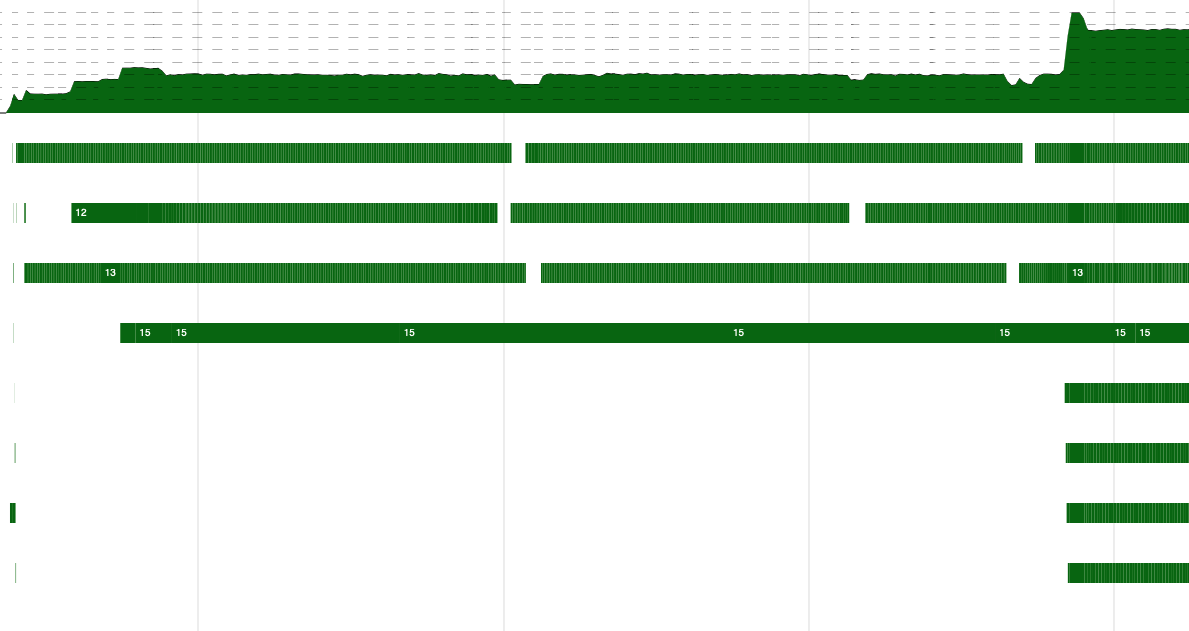
\includegraphics[width=1\linewidth, height=0.2\textheight]{experiments/thread/init}
   \caption{Thread Metrics: Initial execution}
   \label{fig:exp:perf:2}
  \end{minipage}%
  \hspace{.3cm}%
  \begin{minipage}{0.3\textwidth}
    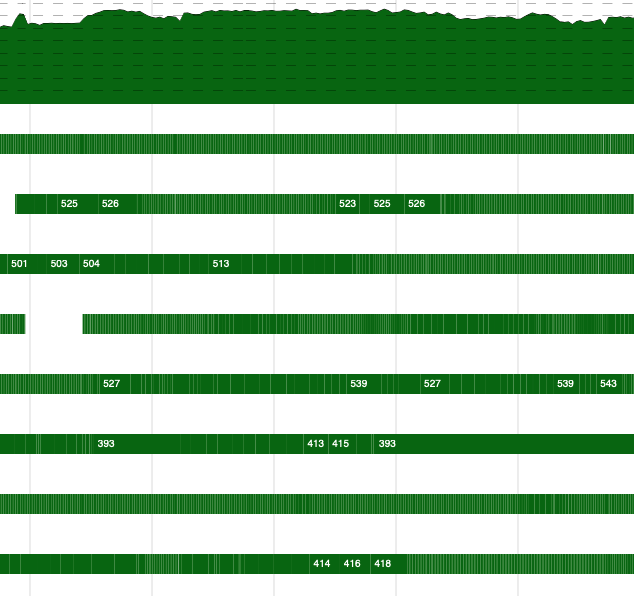
\includegraphics[width=1\linewidth, height=0.2\textheight]{experiments/thread/middle}
    \caption{Thread Metrics: Middle of execution}
    \label{fig:exp:perf:4}
   \end{minipage}% 
   \hspace{.3cm}%
  \begin{minipage}{0.3\textwidth}
   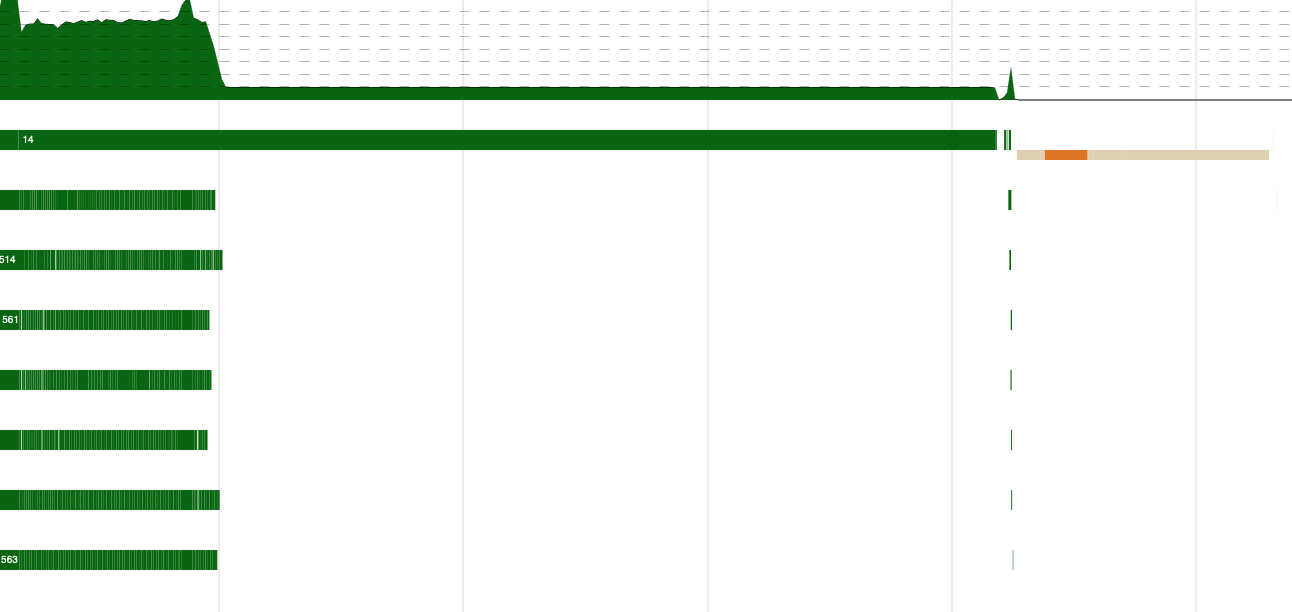
\includegraphics[width=1\linewidth, height=0.2\textheight]{experiments/thread/end}
   \caption{Thread Metrics: End of execution}
   \label{fig:exp:perf:3}
  \end{minipage}%
\end{figure}

\paragraph{Memory Consumption} In the case of memory consumption, we have been able to measure the memory consumption for the biggest graph, \acrshort{dbpedia}. 
As it is known, enabling profiling downgrades performance of execution time, and for this case, the program runs out of memory as we are going to see in the image, but we have still been able to gather interesting data to analyze memory allocation.

\begin{figure}[!htb]
  \begin{center}
     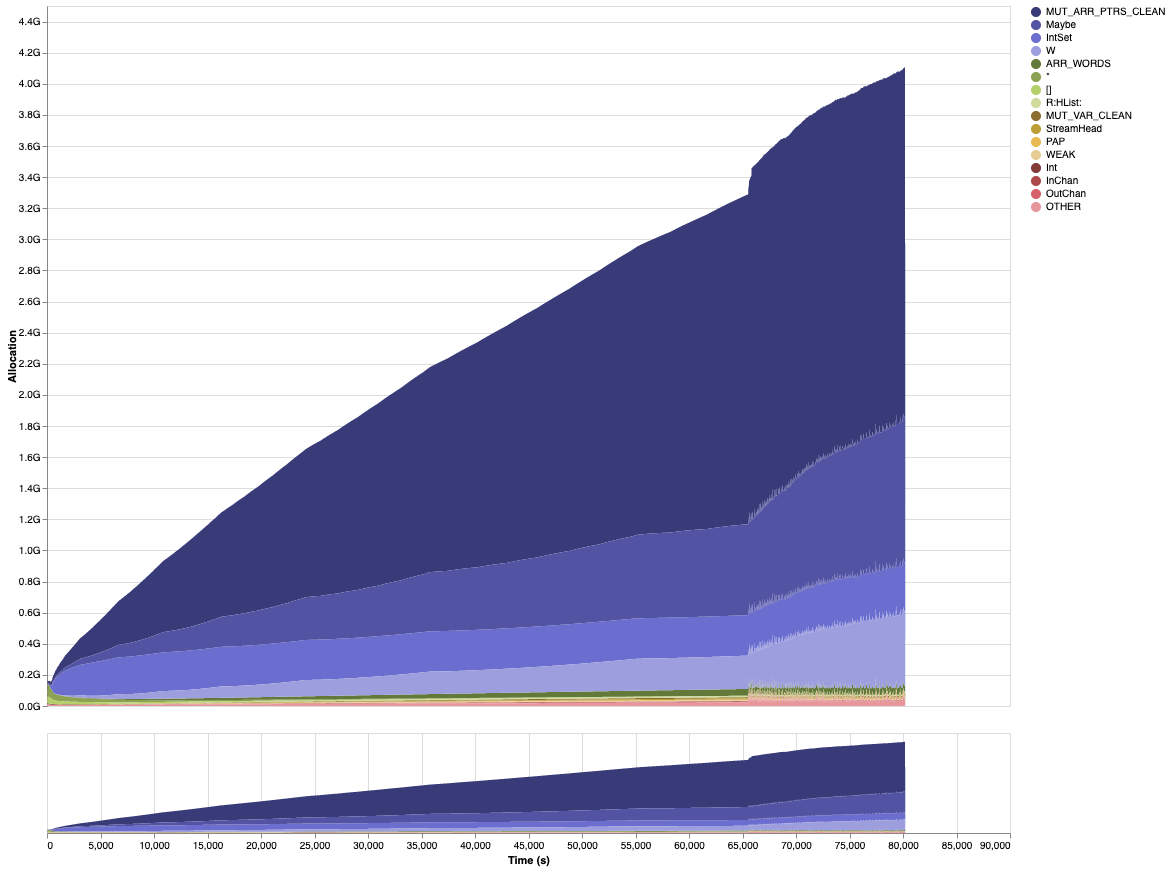
\includegraphics[width=1\textwidth] {experiments/mem/overview}
       \end{center}
     \caption{Memory Metrics: Allocation by Data Type}
     \label{fig:exp:mem:1}
 \end{figure}

As we can appreciate in \autoref{fig:exp:mem:1} the darkest blue space belongs to \mintinline{shell}{MUT_ARR_PTRS_CLEAN}.
This type of objects are pointers to function. In \acrlong{hs} \mintinline{shell}{MUT} (mutator) is the acronym of a thread evaluating a \acrshort{hs} expression.
That means that there are many pointers allocated waiting for evaluating expressions. This is perfectly explained by \acrshort{dp} model, in which we are spawning one
thread per stage, and in particular, that means one thread per filter instance as well. In the case of \acrshort{dbpedia} which contains $168338$ vertices in 
$L$ according to \autoref{table:exp:data-set}, we are spawning the same amount of thread for every run of this network. Since the execution of all these stages will not be released until it finishes the last $\ad$ (processing queries), all of them are waiting for the queries to be processed and executed.
The rest of the memory that is shown in the image is alive data objects such as \mintinline{haskell}{Maybe} and state of the filters instance \mintinline{haskell}{IntSet}. This data is less than $30\%$ of the total allocated memory. The linear growth of the memory could be explained by the reasons exposed before. 
All the $\fbt$ instances are created as long the program executes.

One of the proposed solutions for future work is to reduce the number of $\fbt$ for bigger graphs in order to reduce the number of allocated pointers waiting for commands.

\paragraph{Conclusion E3} We can answer the question [R4] as we have shown that threads are efficiently handled by \acrshort{hs} \acrshort{ghc} scheduler supporting the parallelization level that \acrshort{dp} requires. 
On the other hand, for completely answering the research question regarding memory consumption, although there is a penalty that the program is paying because of the size of the graph and the complexity of the problem, we believe that this aspect can be improved by reducing the number of $\fbt$ instances and choosing suitable data structures used for searching and deliver \acrshort{bt}. 
It was out of the scope of this work to solve the efficiency of the queries, as well as the underlying data structures improvements. 

\section{Chapter Summary}
In this chapter, we have explained in extended detail all the experiments conducted in order to answer the research question exposed.
We first started doing a summary of the research questions. After that, we have presented the setup of the experiments, data, and execution environment details.
Then we have described the experiments, the results, and we have discussed them in deep. At the end of each discussion, we have given a brief conclusion about the observed results and the suitability for answering the pertinent research questions.
